\chapter{REVISÃO DA LITERATURA}

O desenvolvimento de mecanismos que automatizam tarefas existe desde a idade das
pedras, onde hominídeos produziam ferramentas para auxílio próprio. A
transversalidade do conhecimento e da experimentação nos levou a descoberta de
novas metodologias e o aperfeiçoamento de técnicas, consequentemente modificando
a forma com que o ser humano interage com o mundo.

\section{Interfaces gráficas com o usuário}

O conceito de interface é extremamente amplo, e foi largamente difundido com o
início dos estudos de interação humano-máquina. O avanço da industrialização
permitiu com que máquinas extremamente complexas substituíssem seres humanos nas
tarefas mais difíceis, deixando estes, seus operadores, apenas com a
responsabilidade de pilotá-las de forma simples e segura.

O advento de tecnologias multimídias interativas como computadores, celulares e
\textit{tablets} elevou o patamar da criação de interfaces e gestão de tarefas
ao estado da arte, agregando conhecimentos transversais de artistas visuais a
músicos.

\citeonline[p. 1]{ferreira2005semiotics} afirmam que a criação de ``interfaces
com o usuário ainda está mais para arte do que para ciência.'', e justificam,
explicando que ``A maior parte do design ou redesign é baseado em estudos
empíricos ou protótipos, e ainda há muito pouca compreensão teórica ou de
engenharia de como conduzir o processo de design e produzir bons designs pela
primeira vez''.

Interfaces gráficas modernas foram alcançadas através da associação entre
\textit{hardware} e \textit{software}, podendo utilizar de um ou mais
dispositivos de entrada e saída, com o intuito de promover usabilidade e fácil
adaptação.

Dispositivos de entrada transformam coordenadas do mundo real para o mundo
virtual, registrando condições externas que podem ser modificadas através da
interação com um ou mais atores, os usuários. Dispositivos de entrada comuns são
mouse, tela de toque, teclado, etc.

Dispositivos de saída projetam informações geradas por um sistema computacional
e seu caráter é geralmente baseado nos sentidos: Visão, audição, tato. O
dispositivo de saída mais comum é o monitor, que tem por finalidade projetar
imagens compatíveis com a capacidade humana de visão.

\section{Gerenciadores de Janelas}

Gerenciadores de janelas tem como principal função dividir a imagem de um
dispositivo de saída (geralmente monitores) em múltiplas regiões de desenho,
denominadas janelas \cite[p. 5]{myers1996uimss}.

O primeiro conceito acadêmico de gerenciamento de tarefas através da
sobreposição de janelas data de 1969, na tese de Ph.D. de Alan Kay. A
implementação de seu conceito, vista pela primeira vez em funcionamento no
sistema do Xerox PARC, é largamente utilizada até hoje por grandes sistemas
tanto comerciais quanto de código aberto, como Windows, OS X, GNOME, KDE
\cite[p. 7]{myers2000past}.

\tikzstyle{inout}=[draw, fill=blue!20, text width=5em,
    text centered, minimum height=2.5em,drop shadow]
\tikzstyle{other} = [above, text width=5em, text centered]
\tikzstyle{wm} = [inout, text width=10em, fill=red!20,
    minimum height=6em, rounded corners, drop shadow]

\def\blockdist{2.3}
\def\edgedist{2.5}

\begin{figure}[!ht]
  \begin{center}
    \caption{\textbf{Funcionamento de um gerenciador de janelas}}
    \begin{tikzpicture}
        \node (wm) [wm]  {Gerenciador de Janelas};
        \path (wm.west)+(-3.2,1.5) node (app1) [inout] {$Aplicativo$};
        \path (wm.west)+(-3.2,0.5) node (app2)[inout] {$Aplicativo$};
        \path (wm.west)+(-3.2,-1.0) node (dots1)[other] {$\vdots$};
        \path (wm.west)+(-3.2,-2.0) node (app3)[inout] {$Aplicativo$};

        \path (wm.east)+(3.2,1.5) node (monitor1) [inout] {$Monitor$};
        \path (wm.east)+(3.2,0.5) node (monitor2)[inout] {$Televisao$};
        \path (wm.east)+(3.2,-1.0) node (dots2)[other] {$\vdots$};
        \path (wm.east)+(3.2,-2.0) node (monitor3)[inout] {$Projetor$};

        \path [draw, ->] (app1.east) -- node [above] {}
            (wm.160);
        \path [draw, ->] (app2.east) -- node [above] {}
            (wm.180);
        \path [draw, ->] (app3.east) -- node [above] {}
            (wm.200);

        \path [draw, ->] (wm.380) -- node [above] {}
            (monitor1.west);
        \path [draw, ->] (wm.360) -- node [above] {}
            (monitor2.west);
        \path [draw, ->] (wm.340) -- node [above] {}
            (monitor3.west);

        \begin{pgfonlayer}{background}
            \path (app1.west |- app1.north)+(-0.5,0.3) node (a) {};
            \path (wm.south -| wm.east)+(+0.5,-0.3) node (b) {};
            \path (monitor1.east |- monitor3.east)+(+0.5,-0.9) node (c) {};

            \path[fill=yellow!20,rounded corners, draw=black!50, dashed]
                (a) rectangle (c);
            \path (app1.north west)+(-0.2,0.2) node (a) {};

        \end{pgfonlayer}

    \end{tikzpicture}
    \label{window-manager-workflow}
    \fonte{Do Autor (2015)}
  \end{center}
\end{figure}

Um gerenciador de janelas moderno também tem por finalidade coordenar a exibição
de um conjunto de janelas em um conjunto de monitores (conforme fluxograma da
\autoref{window-manager-workflow}), escutar por eventos de entrada (mouse,
teclado) e informar os responsáveis pelas janelas sobre alterações no layout de
tela (dimensões da tela, dimensões da janela, espaço de cor).

Gerenciadores de janelas, porém, não tem por responsabilidade preencher as áreas
de desenho com gráficos, e como suas \textit{Application Programming Interfaces}
(APIs) operam geralmente a nível de pixel, a tarefa de escrever um programa
gráfico acaba sendo demorada e entediante. Além disso, se cada desenvolvedor
criasse seus próprios componentes, seria praticamente impossível disponibilizar
uma experiência consistente ao usuário
\apud{rosenthal1988simple}{myers2000past}.

Através das abstrações disponibilizadas pelos gerenciadores de janelas múltiplas
aplicações gráficas podem coexistir em um mesmo monitor. A construção deste tipo
de aplicação não é de reponsabilidade do gerenciador de janelas, e para isso
ferramentas conhecidas como \textit{toolkits} foram criadas.

\section{\textit{Toolkits} Gráficos}

A principal finalidade de um \textit{toolkit} é viabilizar a interação humano-
computador, permitindo a manipulação direta de elementos gráficos metafóricos,
chamados widgets. Widgets são os componentes funcionais essenciais da interface
gráfica e através deles o usuário pode interagir com programas de computador.

Com seus próprios conjuntos de widgets, \textit{toolkits} possibilitam a criação
de programas com alta consistência visual e comportamental, através da aplicação
de estilo e/ou comportamento próprios nos componentes de interface gráfica com o
usuário \cite{myers2000past}.

As responsabilidades de um \textit{toolkit} vão de desenhar até processar
eventos de um ou mais dispositivos de entrada (mouse, teclado, painel de toque),
verificando a colisão de um evento com um widget (clique em um botão, por
exemplo), traduzindo e informando os eventos para a aplicação proprietária.

Do ponto de vista do programador a finalidade de um \textit{toolkit} é abstrair
características de baixo nível, promovendo a reutilização de código, e
amortizando o custo de desenvolvimento, reduzindo o tempo de desenvolvimento de
novos projetos \cite{haefliger2008code}.

\textit{Toolkits} multiplataforma podem ser utilizados para escrever interfaces
gráficas portáveis, permitindo com que o mesmo código seja compilado para um
sistema operacional diferente do em que foi escrito e funcione da mesma forma.

\section{O \textit{toolkit} GTK+ e a plataforma GNOME}

Existem diversas opções de gerenciadores de janela de código aberto, comumente
incluídos em distribuições de Linux. O GNOME, um ambiente gráfico bastante
difundido pelos usuários de Linux, foi fundado e está em ativo desenvolvimento
por uma comunidade de engenheiros de software ao redor do mundo.

\begin{citacao}
    O GNOME 3 é uma maneira fácil e elegante de usar seu computador.
    Ele foi desenhado para lhe colocar no controle e trazer liberdade para
    todos. O GNOME 3 é desenvolvido pela comunidade GNOME, um grupo
    internacional e diverso de contribuidores que são suportados por uma
    fundação independente, e sem fins lucrativos \cite{gnome-org}.
\end{citacao}

Muito mais que um gerenciador de janelas, a experiência GNOME é construída por
um conjunto de aplicações centrais, que incluem um gerenciador de janelas, um
lançador de aplicações e diversos aplicativos centrais, como calculadora,
editor de texto, gerenciadores de arquivos, redes, contatos, etc.

\begin{figure}[!ht]
  \begin{center}
    \label{mclasen-new-apps}
    \caption{\textbf{Uma captura de tela do GNOME 3.16}}
    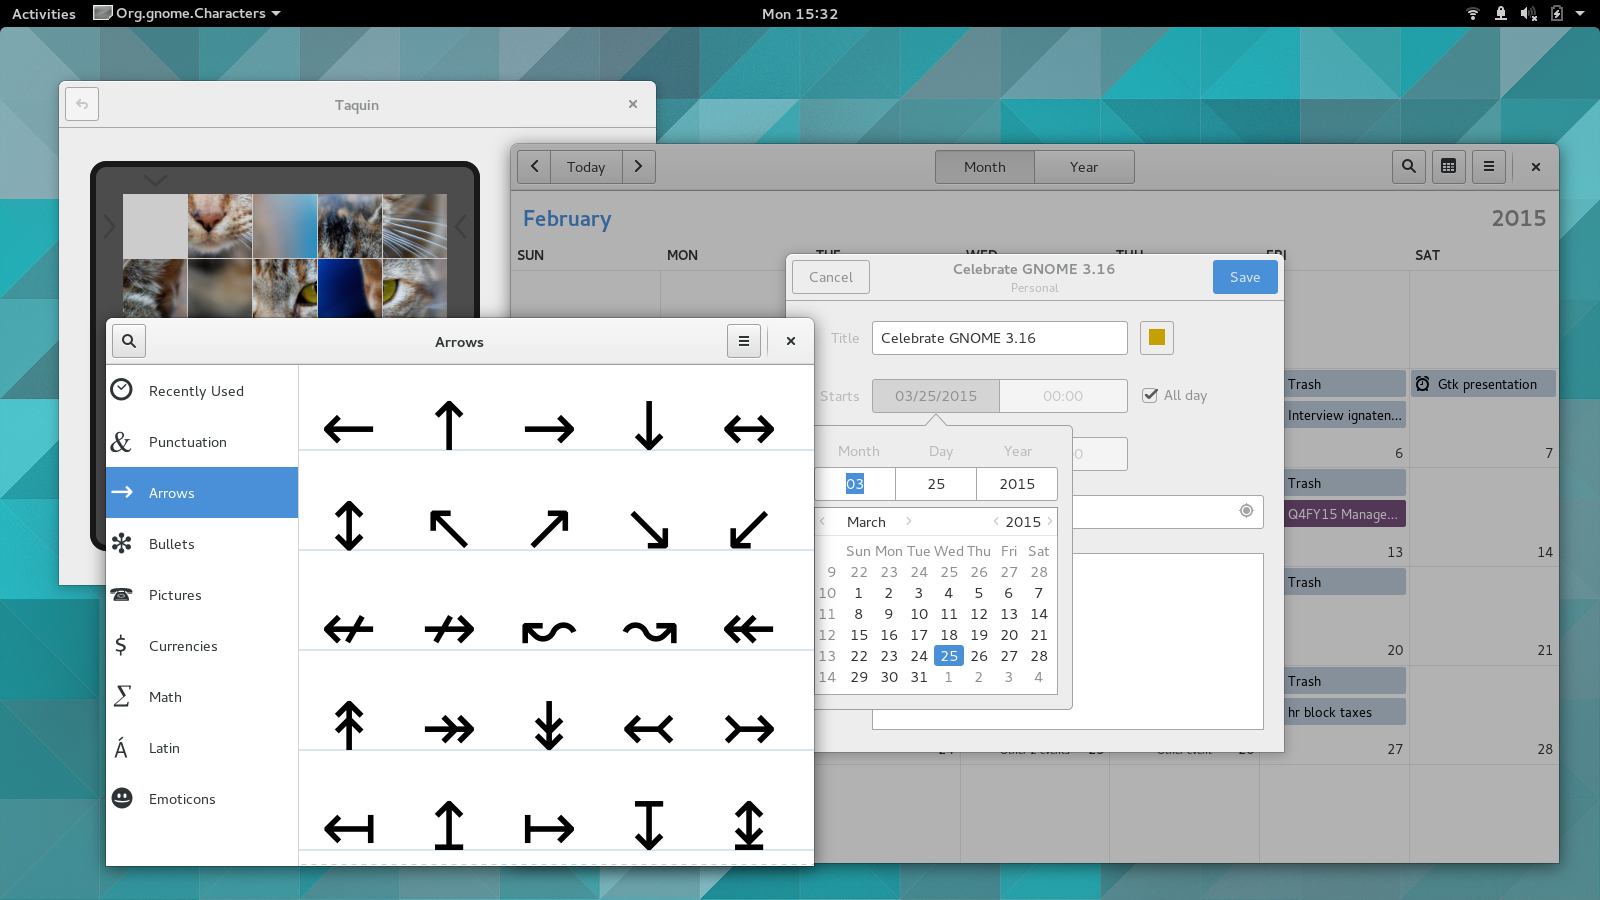
\includegraphics [width=\textwidth]{image/mclasen-new-apps.png}
    \fonte{\cite{gnome316mclasen}}
  \end{center}
\end{figure}

A plataforma GNOME e seus aplicativos centrais são baseados no \textit{toolkit}
GTK+. O GTK+ é formado por um conjunto de ferramentas multi-plataforma para
criar interfaces gráficas de usuário. Por oferecer um conjunto completo de
widgets é adequado para projetos desde pequenas ferramentas pontuais até suítes
completas de aplicativos \cite{gtk-org}.

\section{Software livre e o desenvolvimento contínuo}

Uma das característica das plataformas de código aberto é a distribuição de
esforços em prol do constante desenvolvimento e melhoria. A pluralidade de
opiniões e idéias eleva o patamar das discussões e permite com que vários pontos
de vista sejam levados em consideração na evolução da plataforma.

Apesar dos prós existentes na distribuição de esforços também existem os contras
-- Projetos que são desenvolvidos paralelamente nem sempre avançam na mesma
velocidade. O contra fica mais sério quando um projeto depende do outro, como é
o caso de \textit{toolkits} e programas que consomem suas APIs.

Quando ocorrem mudanças na interface de programação de uma framework ou
biblioteca, softwares dependentes tem de se adaptar as mudanças. O efeito
cascata provocado pela propagação de alterações na malha de softwares
dependentes não é incomum, e já foi objeto de estudo \cite{yau1978ripple}.

\section{Impactos na consistência e usabilidade}

Além dos aplicativos centrais, geralmente garantidos de acompanhar a evolução
da plataforma -- sua ergonomia e visual -- existe uma vasta gama de aplicações
tanto de código aberto quanto proprietárias disponíveis para atender as mais
variadas necessidades.

A grande maioria das aplicações GTK+ são mantidas pela comunidade de software
livre, e se não atualizadas podem ficar defasadas em usabilidade, ergonomia e
consistência com a plataforma. \citeonline{shneiderman1992designing} descreve
a usabilidade como uma combinação das seguintes características:

\begin{itemize}
    \item Facilidade de aprendizado
    \item Alta velocidade de operação
    \item Baixa taxa de erros
    \item Satisfação do usuário
    \item Retenção de usuários pelo tempo
\end{itemize}

Em prol da usabilidade a maioria dos \textit{toolkits} aplica um modelo próprio
de apresentação, organização, interação e estilização de widgets, atendendo aos
requisitos do tipo de ambiente onde é executado (desktop, tablet e celular).

\section{HIG ou Human Interface Guidelines}

Divulgado no ano de 2014, acompanhando a versão 3.14 da plataforma GNOME, sob o
título de \textit{Human Interface Guidelines}, o conjunto de padrões de design
oficialmente promovido pela GNOME Foundation busca promover a máxima integração
de interfaces gráficas GTK+ na plataforma GNOME.

\begin{citacao}
    Se você é um desenvolvedor com experiência limitada de design o HIG foi
    planejado para auxiliar você a criar facilmente uma interface de usuário
    efetiva. Para designers, o HIG provê uma introdução as possibilidades ao
    usar o GTK+, assim como padrões de design que são usados nos aplicativos
    GNOME \cite{gnome314hig}.
\end{citacao}

O HIG, como também é chamado, é uma literatura ilustrada de diretrizes
recomendadas no desenvolvimento de interfaces gráficas que utilizem o
\textit{toolkit}, com o intuito de reforçar a consistência visual e integração
com o ambiente GNOME. A figura \ref{gnome-hig-patterns} ilustra alguns dos
padrões de design documentados pelo HIG.

\begin{figure}[!ht]
  \begin{center}
    \caption{\textbf{Padrões e suas aplicações}}
    \label{gnome-hig-patterns}
    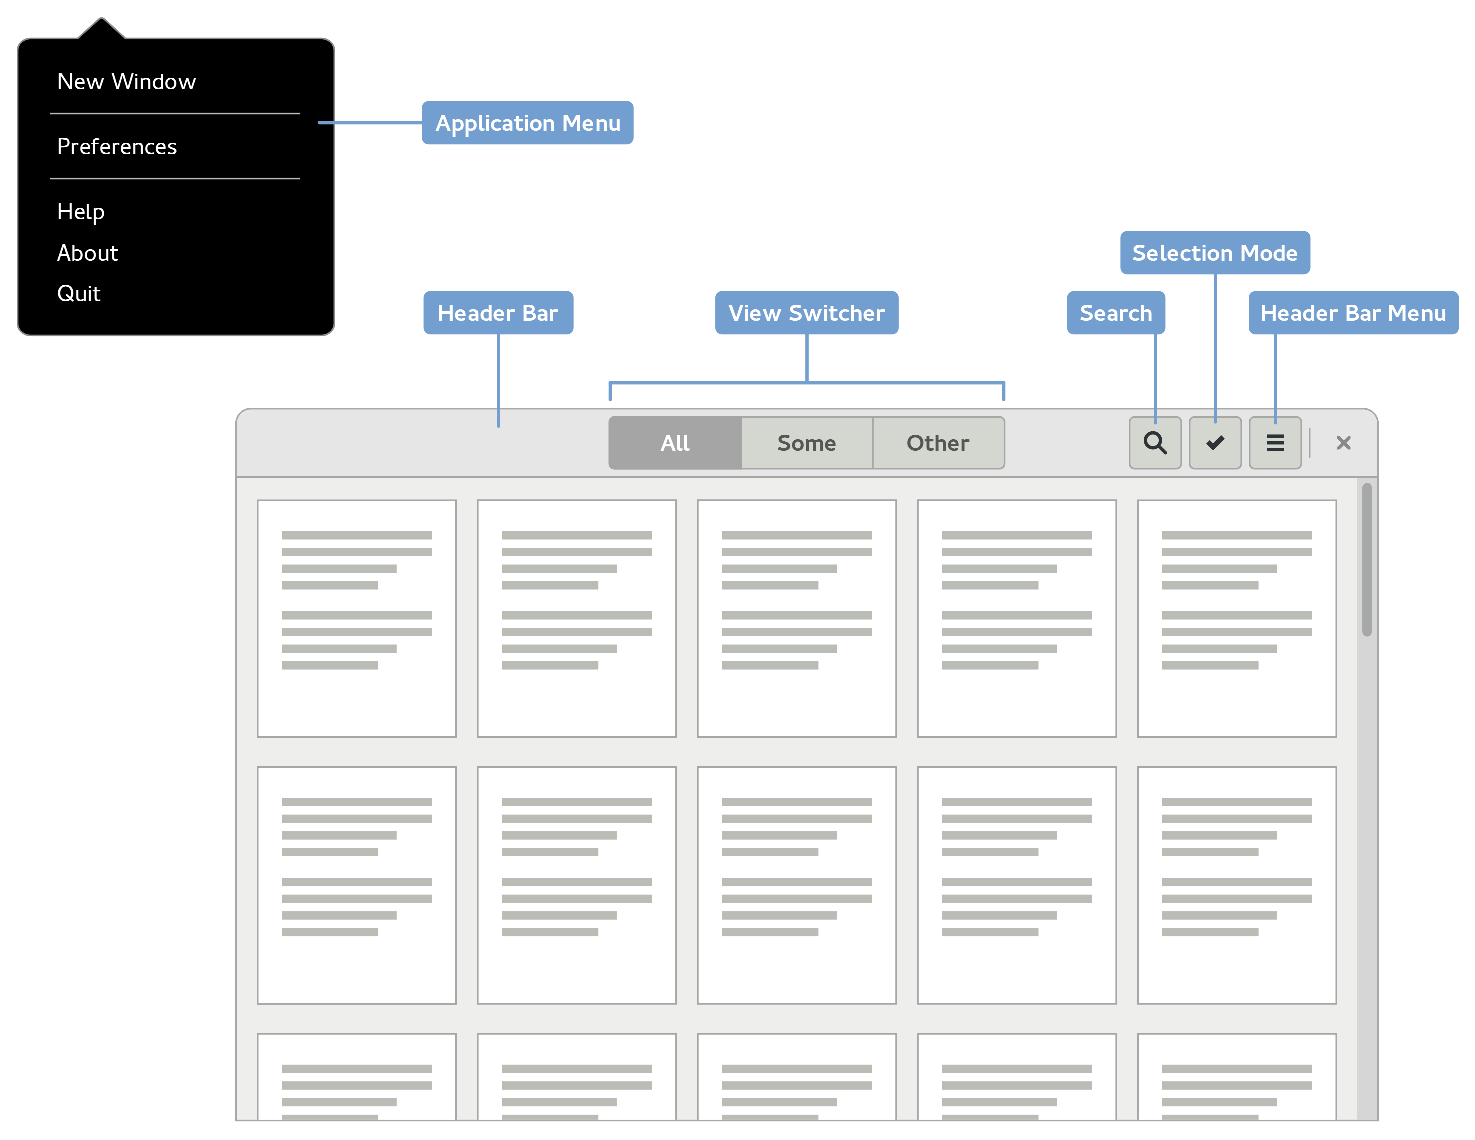
\includegraphics[width=\textwidth]{image/hig/patterns.eps}
    \fonte{\cite{hig314patterns}}
  \end{center}
\end{figure}

Dentre os objetivos do HIG estão a transmissão das metas de design de alto nível
e estratégicas da experiência GNOME e a comunicação das diretrizes de design
essenciais, de uma forma clara e viva, acompanhando a evolução da plataforma.

\section{Estudo de caso: Transmission}

Um aplicativo famoso disponível para a plataforma GNOME é o cliente de
\textit{BitTorrent} Transmission \cite{transmission282}. Aclamado pela sua
simplicidade, o aplicativo é utilizado para compartilhar arquivos através da
internet.

Utilizando-se de uma configuração padrão funcional e poucos cliques para
configurar funcionalidades avançadas a utilização do cliente de torrent
Transmission foi projetada para ser fácil e poderosa
\cite{transmission-about}.

A primeira versão do Transmission foi lançada em Setembro de 2005, já com uma
interface gráfica baseada em GTK+, projetada sob as recomendação do HIG
da época, publicada digitalmente em formato de livro \cite{gnome221hig}.

\begin{figure}[!ht]
  \begin{center}
    \caption{\textbf{Transmission 2.28 no GNOME 3.16}}
    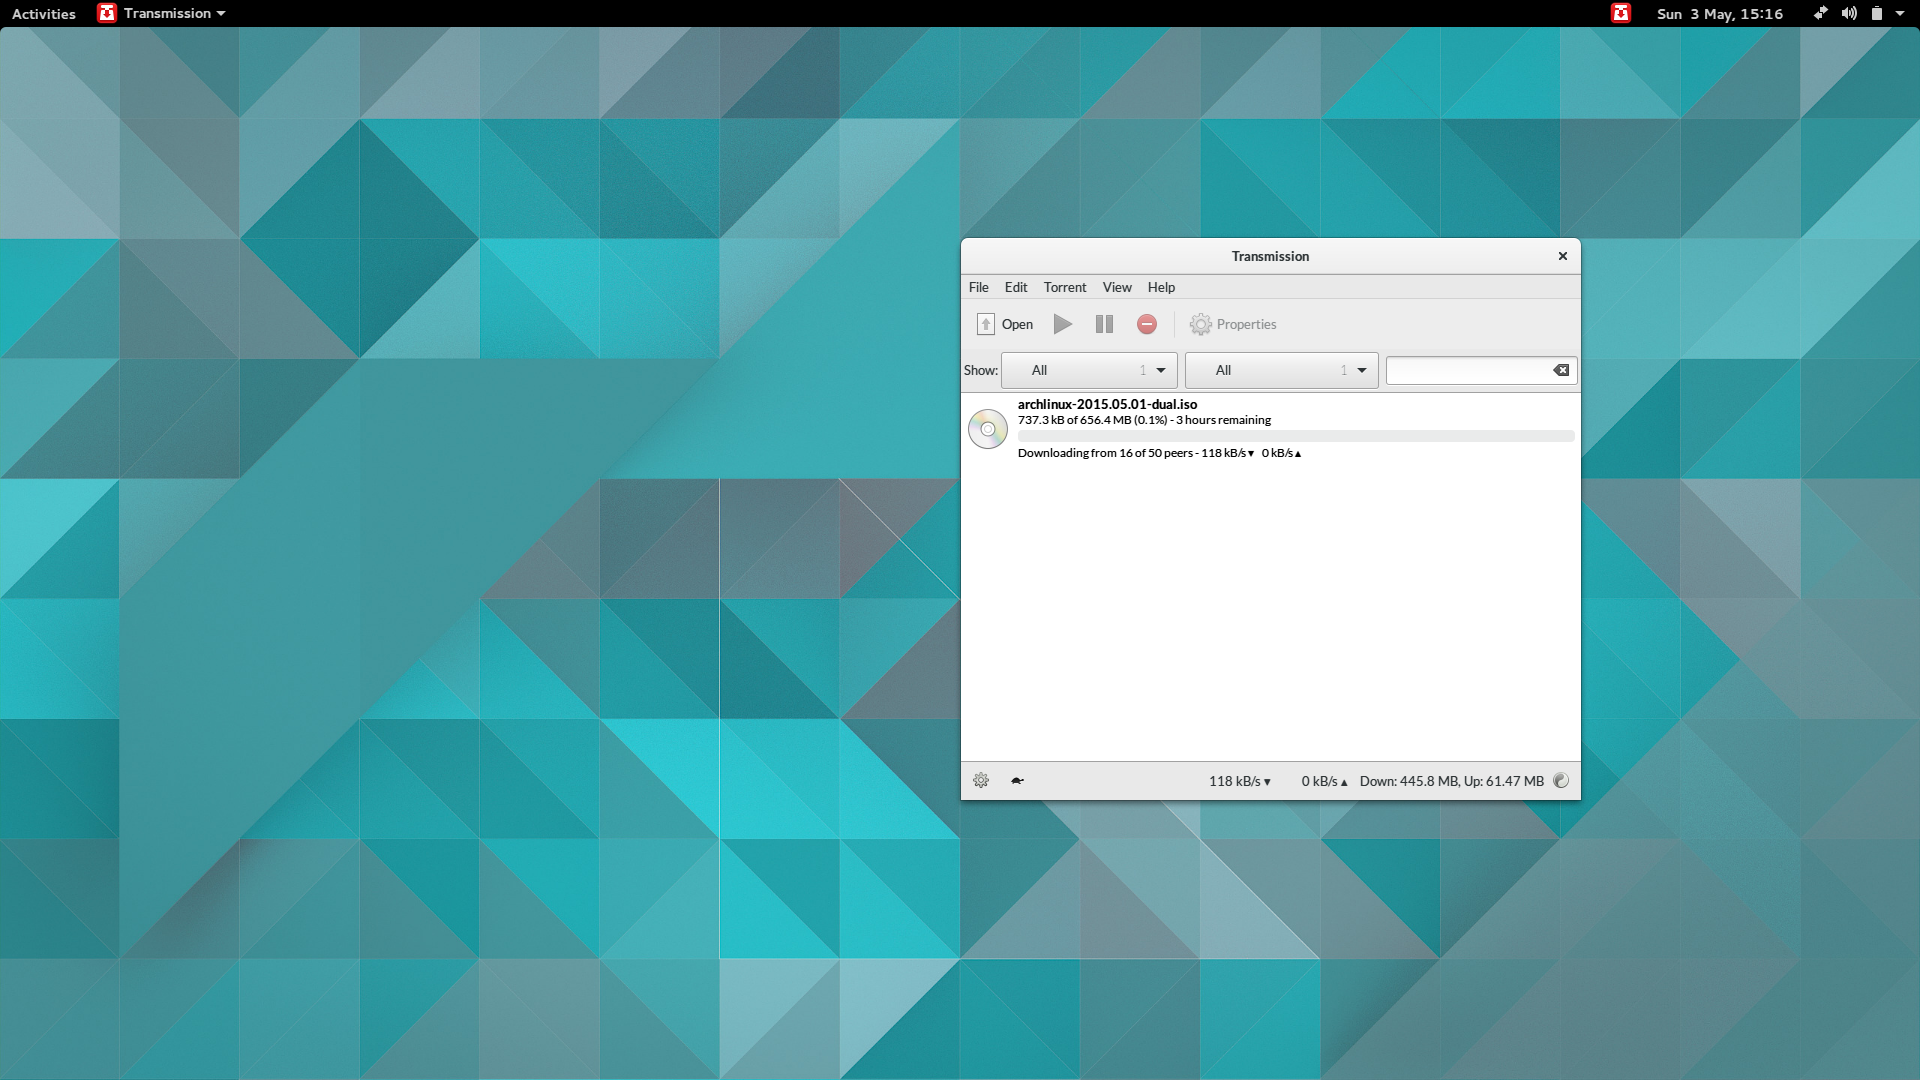
\includegraphics [width=\textwidth]{image/transmission/282-master/main-window.png}
    \label{transmission-master}
    \fonte{Do Autor (2015)}
  \end{center}
\end{figure}
